\documentclass[11pt]{article}
\usepackage{fullpage}
\usepackage{amsthm}
\usepackage{amsmath} \usepackage{amssymb}
\usepackage{graphicx}

\graphicspath{ {./imgs/} }

\setlength{\parindent}{0pt}

\title{Distributed Algorithms (CO347)}
\author{Michael Tsang}

\newtheorem{defn}{Definition}
\newtheorem{eg}{Example}
\newtheorem{theo}{Theorem}
\newtheorem{lem}{Lemma}

\begin{document}

\maketitle
\section{Motivation}
\subsection{Why a Distributed System?}
\begin{itemize}
  \item Computation and data distribution.
  \item Performance through parallelisation and distribution.
  \item Reliability and availability through replication, fault-tolerance, security.
  \item Scalability, modularity, evolvability.
  \item Heterogenity of hardware and software.
\end{itemize}

\subsection{What is a Distributed System?}
\begin{itemize}
  \item A set of processes connected by a network.
    \begin{itemize}
      \item Machines can be located across the planet.
      \item Communicate via message passing, no shared memory.
    \end{itemize}
  \item No common physical clock.
    \begin{itemize}
      \item No total order on events by time.
    \end{itemize}
\end{itemize}

\subsection{Assumptions}
When designing distributed systems, we have to consider different assumptions.

\subsubsection{Timing}
\begin{itemize}
  \item \textbf{Synchronous systems}:
    \begin{itemize}
      \item Upper bound on process delays.
      \item Upper bound on time for a message to be delivered.
      \item Can translate results to asynchronous models.
    \end{itemize}
  \item \textbf{Asynchronous systems}:
    \begin{itemize}
      \item Processes and communication take arbitrary time.
      \item No assumption that processes have physical clocks, but can be useful to use logical clocks.
    \end{itemize}
  \item \textbf{Partially synchronous systems}:
    \begin{itemize}
      \item Real-world systems are mostly synchronous with asynchronous periods.
      \item Assume the system is eventutally synchronous.
    \end{itemize}
\end{itemize}

\subsubsection{Failures}
\begin{itemize}
  \item \textbf{No failures}:
    \begin{itemize}
      \item Unrealistic.
    \end{itemize}
  \item \textbf{Process failure}:
    \begin{itemize}
      \item e.g.\ software bugs; OS/user termination; OS failure.
      \item Process stops sending messages it is supposed to send.
      \item Process sends messages it is not supposed to send.
    \end{itemize}
  \item \textbf{Link failure}:
    \begin{itemize}
      \item e.g.\ cable, router, wireless, adversary.
      \item Inter-process communication failure, e.g.\ non-delivery of messages; corrupt messages; duplicates.
      \item Need for reliable protocols and secure channels.
      \item Partitioned networks.
    \end{itemize}
\end{itemize}

\subsubsection{Failure Classes}
\begin{itemize}
  \item \textbf{Process crash failure} (crash-stop failure):
    \begin{itemize}
      \item Process halts and does not perform further action.
      \item Different types:
        \begin{itemize}
          \item \textbf{Fail-stop} - can be reliably detected by other processes.
          \item \textbf{Fail-silent} - cannot be reliably detected.
          \item \textbf{Fail-noisy} - detection takes time.
          \item \textbf{Fail-recovery} - crashed processes can recover
        \end{itemize}
      \item Non-faulty processes are a \textbf{correct process}.
    \end{itemize}
  \item \textbf{Link failure}:
    \begin{itemize}
      \item Link goes down and stays down.
      \item Network may partition or remain connected.
    \end{itemize}
  \item \textbf{Omission failure}:
    \begin{itemize}
      \item Two types:
        \begin{itemize}
          \item \textbf{Send omission} - does not send all required messages.
          \item \textbf{Receive omission} - does not receive all require messages.
        \end{itemize}
    \end{itemize}
  \item \textbf{Byzantine failure} (fail-arbitrary):
    \begin{itemize}
      \item Arbitrary (or malicious) behaviour.
    \end{itemize}
\end{itemize}

\subsubsection{Communication}
\begin{itemize}
  \item \textbf{Asynchronous message passing}:
    \begin{itemize}
      \item The process sending a message continues after sending.
      \item We can build a \textbf{synchronous message passing} mechanism, e.g.\ process waits until message is delivered to the receiving process.
      \item We can build a \textbf{shared memory abstraction}.
    \end{itemize}
  \item \textbf{Reliable message communication}:
    \begin{itemize}
      \item Assume that messages sent using reliable protocol.
      \item Communications can still fail.
      \item Use TCP to send messages, simulate network failure by dropping messages in software.
    \end{itemize}
  \item \textbf{Message delays are bounded}:
    \begin{itemize}
      \item Processes timeout if message is delayed too long.
    \end{itemize}
\end{itemize}

\section{Reliable Broadcast}
We discuss algorithms for reliable broadcast in \textbf{asynchronous message-passing} distributed systems that are subject to \textbf{process failure}, we want:
\begin{itemize}
  \item To guarantee that messages are consistently delivered to processes.
  \item Agreement on delivered messages.
  \item No ordering among delivered messages.
\end{itemize}

\subsection{Structure}
Each distributed process is a set of interconnected components.
Each distributed process will typically have the same set of components.

\begin{figure}[htb!]
  \centering
  \caption{Elixir mappings.}
  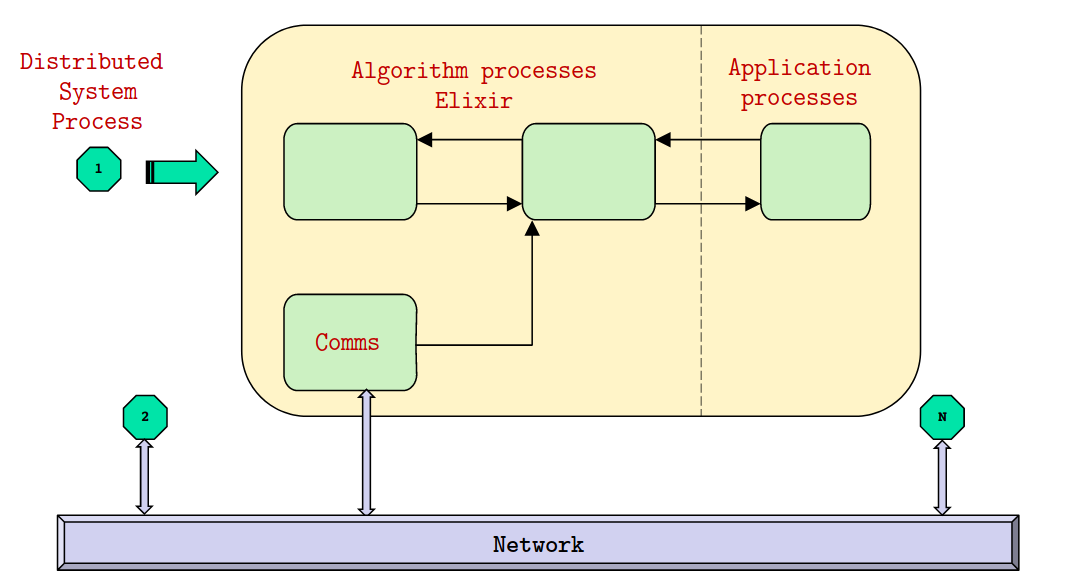
\includegraphics[scale=0.3]{elixirmapping}
\end{figure}

We implement this in \textit{Elixir} where a distributed system process is 1 \textit{Elixir} node, which is many \textit{Elixir} processes.
The components are \textit{Elixir} processes which use message passing for intra-node interactions

\subsection{Assumptions}
\begin{itemize}
  \item \textbf{Asynchronous system}:
    \begin{itemize}
      \item No bound on message delays.
      \item No bound on time to execute a local process step.
      \item Time to execute a step is finite.
    \end{itemize}
  \item Processes interact by \textbf{message passing}.
  \item \textbf{Message passing is reliable}.
  \item Every process can logically communicate with every other.
  \item Number of processes fixed and known.
  \item Crashed processes do not continue.
\end{itemize}

\subsection{Classes of Broadcast}
\begin{itemize}
  \item \textbf{One shot} - each message is considered separately from others:
    \begin{itemize}
      \item Best-Effort Broadcast (BEB).
      \item Reliable Broadcast (RB).
      \item Uniform Reliable Broadcast (URB).
    \end{itemize}
  \item \textbf{Multishot} - involve all messages that are broadcast:
    \begin{itemize}
      \item FIFO Message delivery.
      \item Casual Order Message Delivery.
      \item Total Order Message Delivery.
    \end{itemize}
\end{itemize}

\subsection{Perfect Point-to-Point Links (PL)}
The distributed processes communicate with PL components.
\begin{figure}[htb!]
  \centering
  \caption{Perfect point-to-point links component.}
  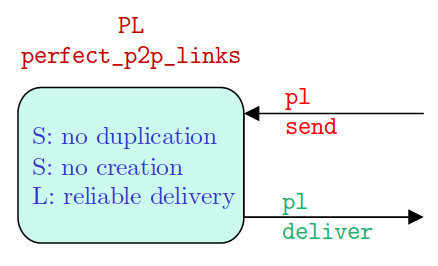
\includegraphics[scale=0.3]{pl}
\end{figure}

\subsubsection{Safety and Liveness Properties}
\begin{itemize}
  \item \textbf{Reliable Delivery (L)} - if Alice and Bob are correct processes, then every message sent by Alice to Bob is eventually delivered to Bob.
  \item \textbf{No Duplication (S)} - no message is delivered to a process more than once.
  \item \textbf{No Creation (S)} - no message is delivered unless it was sent.
\end{itemize}

\subsection{Best-Effort Broadcast (BEB)}
Given a list of all processes and a message, we send the message to all processes (including ourselves) with multiple sends:
\begin{itemize}
  \item If sending is reliable, then every correct process will receive a copy, crashed processes may or may not have received a copy.
  \item The messages will be received at arbitrary times.
  \item If the sending process crashes during broadcast, some arbitrary subset of processes will receive the message.
  \item The sender does not know which processes have received the message.
\end{itemize}

\begin{figure}[htb!]
  \centering
  \caption{Best-effort broadcast component.}
  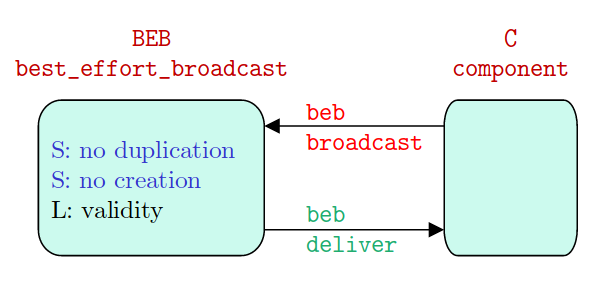
\includegraphics[scale=0.3]{beb}
\end{figure}

We assume messages are unique (e.g.\ they include a process-id and seq-no), no process broadcasts a message twice, and no two processes every broadcast the same message.

\subsubsection{Safety and Liveness Properties}
\begin{itemize}
  \item \textbf{Validity (L)} - if a correct process broadcasts a message, then every correct process eventually delivers it.
  \item \textbf{No Duplication (S)} - no message is delivered to a process more than once.
  \item \textbf{No Creation (S)} - no message is delivered unless it was broadcast.
\end{itemize}

\subsection{BEB Basic Broadcast}
\begin{figure}[htb!]
  \centering
  \caption{Basic broadcast.}
  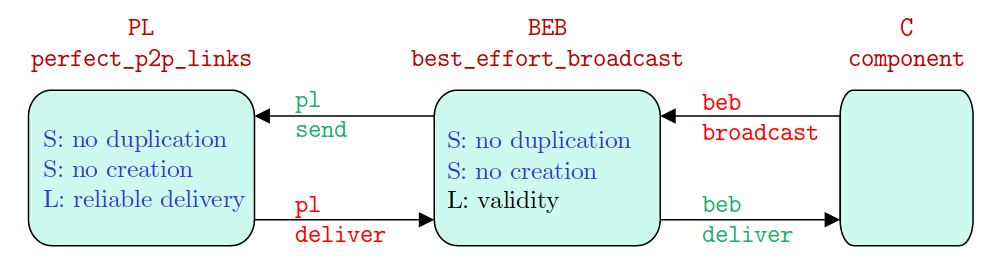
\includegraphics[scale=0.3]{bebpl}
\end{figure}

\begin{itemize}
  \item BEB sends a message to each process using the PL component - this works as PL ensures all correct processes deliver messages, as long as the sender does not crash.
  \item BEB is fail-silent.
  \item $1$ broadcast step and $O(N)$ messages, where $N$ is the number of processes.
  \item BEB derives its S\&L properties from PL.
\end{itemize}

\subsubsection{Safety and Liveness Properties}
\begin{itemize}
  \item \textbf{No Duplication (S)} and \textbf{No Creation (S)} dervied from PL.
  \item \textbf{No Duplication (S)} also assumes messages are unique.
  \item \textbf{Validity (L)} derived from \textbf{Reliable Delivery (L)} in PL and the fact that the message needs to be sent to all processes.
\end{itemize}

\subsection{Reliable Broadcast (RB)}
\begin{figure}[htb!]
  \centering
  \caption{Reliable broadcast component.}
  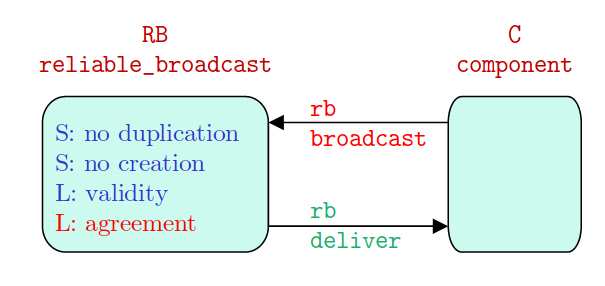
\includegraphics[scale=0.3]{rb}
\end{figure}
All correct processes will agree on the messages they deliver, even if the broadcasting process crashes while sending.

\subsubsection{Safety and Liveness Properties}
\begin{itemize}
  \item \textbf{Validity (L)}, \textbf{No Duplication (S)}, and \textbf{No Creation (S)} as in BEB.
  \item \textbf{Agreement (L)}:
    \begin{itemize}
      \item If a correct process delivers message $M$, then every correct process also delivers $M$.
      \item Validity and Agreement together provide a \textbf{Termination} property for broadcasting a message.
      \item Faulty process could deliver messages not delivered by correct processes.
    \end{itemize}
\end{itemize}

\subsection{Eager RB (fail-silent)}
\begin{figure}[htb!]
  \centering
  \caption{Eager RB.}
  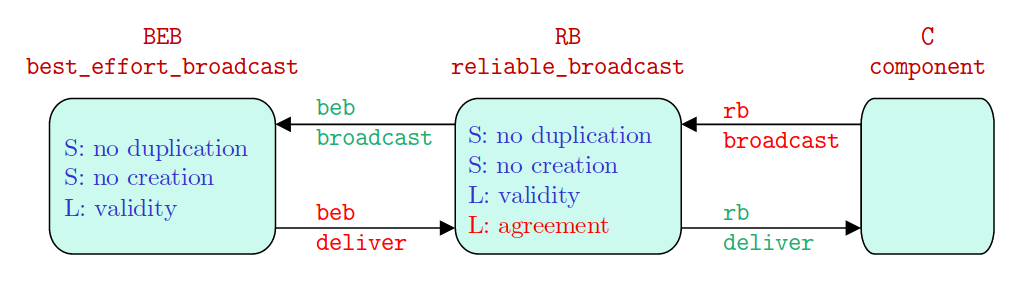
\includegraphics[scale=0.3]{rbbeb}
\end{figure}

\begin{itemize}
  \item Every process re-broadcasts every message it delivers.
  \item If the broadcasting process crashes, then the message will be forwarded by other processes using BEB.
  \item At best $1$ broadcast step, at worst $O(N)$ broadcast steps if processes crash in sequence.
  \item $O(N^2)$ messages.
\end{itemize}

\subsubsection{Safety and Liveness Properties}
\begin{itemize}
  \item \textbf{No Creation (S)} and \textbf{Validity (L)} derived from BEB.
  \item \textbf{No Duplication (S)} as messages delivered are kept track of, and messages are assumed to be unique.
  \item \textbf{Agreement (L)} is derived from \textbf{Validity (L)} of BEB, and the fact that every correct process forwards every message it delivers.
\end{itemize}

\subsection{Lazy RB (fail-stop)}
\begin{figure}[htb!]
  \centering
  \caption{Lazy RB.}
  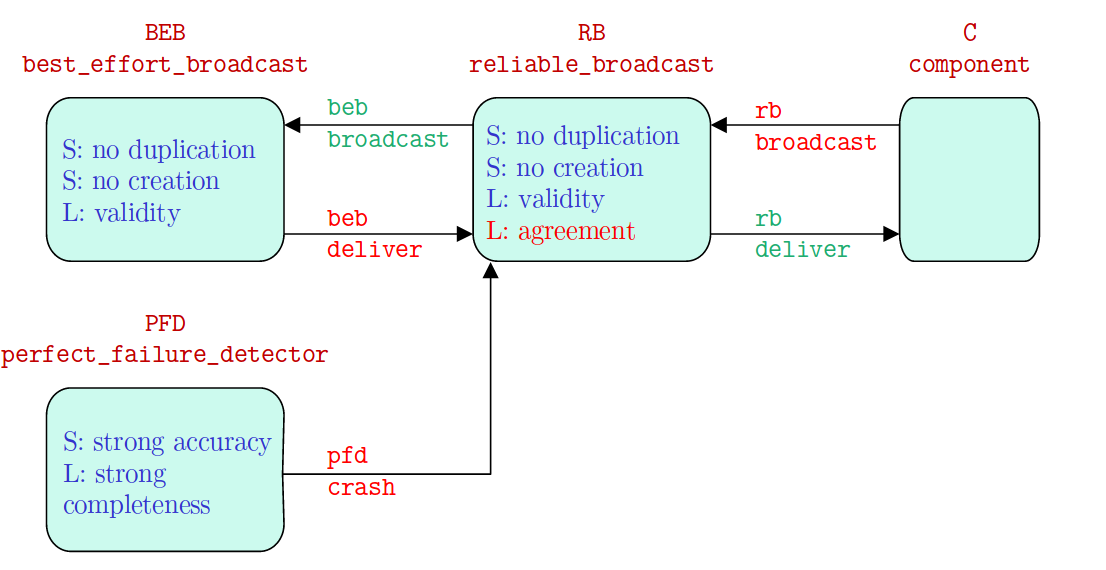
\includegraphics[scale=0.3]{lazyrb}
\end{figure}

\begin{itemize}
  \item Uses BEB, but includes a failure detector component to detect processes that have failed (and stopped).
  \item When a crash is detected, all messages from that process are broadcast.
  \item When a messsage is received from a crashed process then the message is broadcast, otherwise if it is a correct process it is not.
\end{itemize}

\subsubsection{Safety and Liveness Properties}
\begin{itemize}
  \item \textbf{Agreement (L)} is derived from the \textbf{Validity (L)} from BEB, that every correct process forwards every message it delivers when it detects a crashed process, and from PFD.
  \item Other properties follow as for the Eager RB.
\end{itemize}

\subsection{Failure Detectors}
\begin{itemize}
  \item \textbf{Perfect Failure Detector} $P$:
    \begin{itemize}
      \item Provides processes with a list of suspected (detected) processes that have crashed.
      \item Makes timing assumptions (assumes systems are not asynchronous).
      \item Never changes its view - suspects remain suspected forever.
    \end{itemize}
  \item \textbf{Eventually Perfect Failure Detecter}: $\Diamond P$:
    \begin{itemize}
      \item May make mistakes but will eventually detect a crashed process.
    \end{itemize}
\end{itemize}

\subsubsection{Safety and Liveness Properties}
\begin{itemize}
  \item \textbf{Strong Completeness (L)} - every process that crashes will eventually be permanently suspected by every correct process.
  \item \textbf{Strong Accuracy (S)} - no process is suspected before it crashes.
  \item \textbf{Eventually Strong Accuracy (L)} - eventually no correct process is suspected.
\end{itemize}

\subsection{PFD Exclude on Timeout}
\begin{figure}[htb!]
  \centering
  \caption{Exclude on timeout.}
  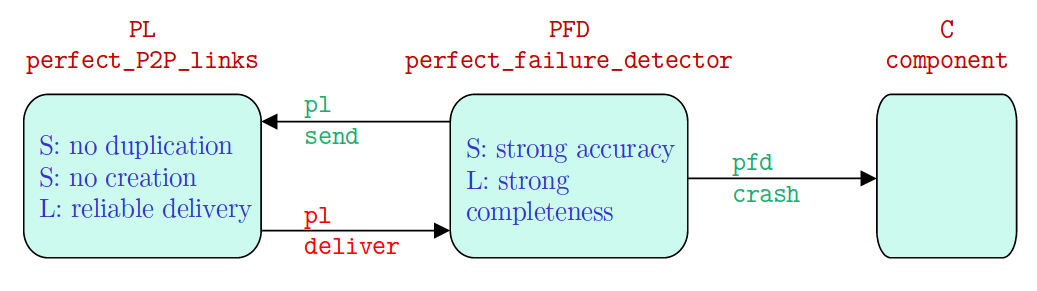
\includegraphics[scale=0.3]{pfd}
\end{figure}

\begin{itemize}
  \item Uses PL to exchange \textit{heartbeat} messages with a timeout mechanism.
  \item Timeout delay must be large enough for all sends to processes, processing time, and replies back.
  \item After timeout, processes from which a reply has not been received are considered crashed, even if it is alive and the reply arrived after timeout.
\end{itemize}

\subsubsection{Safety and Liveness Properties}
\begin{itemize}
  \item \textbf{Strong Completeness (L)}:
    \begin{itemize}
      \item If a process crashes, it stops replying to heartbeat messages; no process will deliver its reply.
      \item PL ensures no message is delivered unless sent.
      \item Then every correct process will detect the crash.
    \end{itemize}
  \item \textbf{Strong Accuracy (S)}:
    \begin{itemize}
      \item A process is suspected only if no reply is delivered before timeout.
    \end{itemize}
\end{itemize}

\subsection{Process Configuration}
Each distributed process is in the configuration seen in figure \ref{fig:processconf}.

\begin{figure}[htb!]
  \centering
  \caption{Full configuration of a distributed process.}
  \label{fig:processconf}
  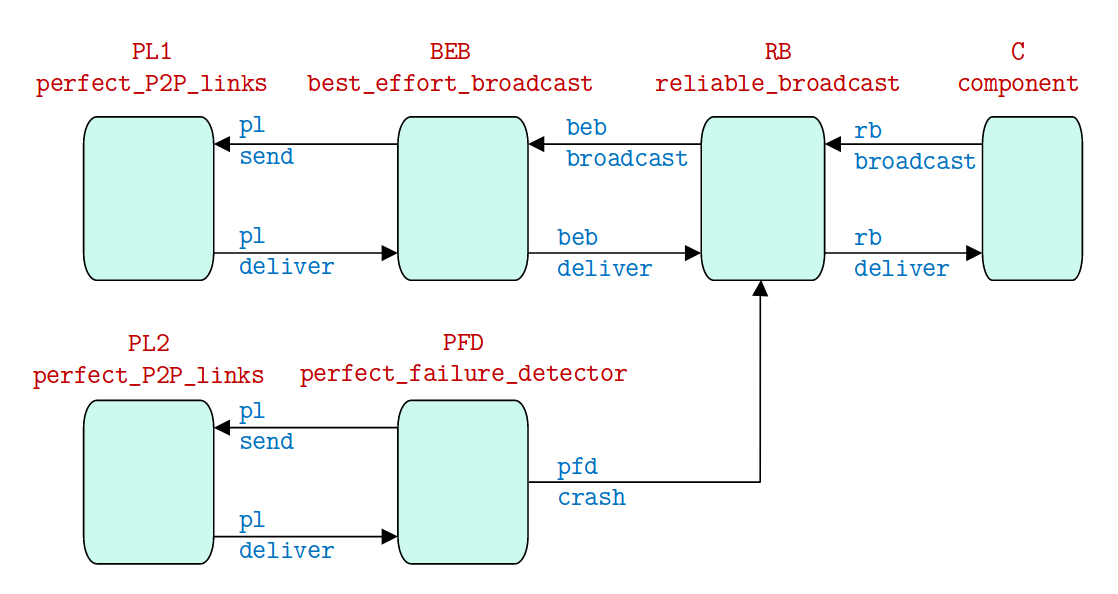
\includegraphics[scale=0.3]{processconf}
\end{figure}

\subsection{Uniform Reliable Broadcast (URB)}
\begin{figure}[htb!]
  \centering
  \caption{Uniform reliable broadcast.}
  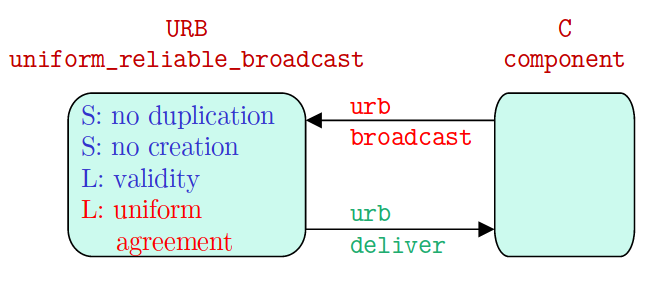
\includegraphics[scale=0.3]{urb}
\end{figure}

\begin{itemize}
  \item \textbf{Validity (L)}, \textbf{No Duplication (S)}, and \textbf{No Creation (S)} are the same as for BEB and RB.
  \item \textbf{Uniform Agreement (L)}:
    \begin{itemize}
      \item If a process (not necessarily correct) delivers a message $M$, then every correct process will also deliver $M$.
      \item The set of messages delivered by a faulty process is always a subset of messages delivered by a correct process.
    \end{itemize}
\end{itemize}
\end{document}
